\chapter{Future prospects}
\label{chapter:koopmans_bernardi}

\begin{bf}
  \author{Leon V. E. Koopmans (Kapteyn Astronomical Institute), Gianni Bernardi (INAF-IRA \& Rhodes University)}\\
  
Abstract\\
\end{bf}

This chapter discusses some important things




\section{Forthcoming interferometric ground based instruments and upgrades}

In this section we review the status of the 21~cm ground based interferometers that are under construction, have been upgraded or will be constructed in the near future.

\subsection{The Hydrogen Epoch of Reionization Array}
\begin{figure}[]
\begin{center}
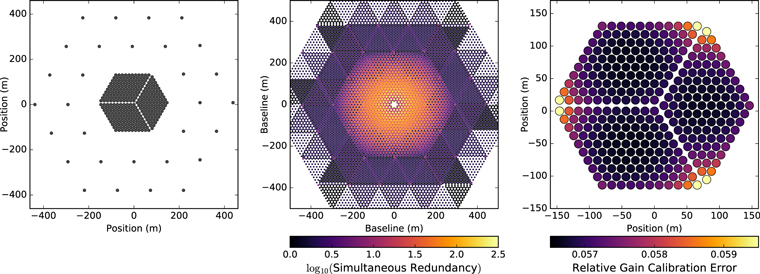
\includegraphics[width=1.\textwidth]{Koopmans_Bernardi/hera_layout}
\end{center}
\caption{The HERA layout (left panel): 320~dishes are located in the hexagonal core and 30 more outrigger dishes are planned to be deployed out to a maximum baselines of $\sim 800$~m to improve angular resolution and imaging capabilities. The core is split in three sectors that are displaced from each other by a fraction of the dish diameter (see \cite{dillon16} for a detailed discussion. The split core provides a significantly improved instantaneous $uv$ coverage (central panel) whilst retaining high redundancy. The right panel shows the expected relative antenna gain errors after using redundant calibration (from \cite{dillon16}).}
\label{fig:fig_hera}
\end{figure}
The Hydrogen Epoch of Reionization Array (HERA, \cite{deboer17}) is an array currently under construction in the Karoo reserve area in South Africa - following the decommissioning of the PAPER experiment (see Chapters~\ref{chapter:bernardi} and 8 in this book for an overview of PAPER). HERA is built following the approach used for PAPER: a highly redundant array to maximize the sensitivity on a number of power spectrum modes measured using the avoidance approach. In order to increase the sensitivity with respect to PAPER, it employs 14~m diameter non steerable dishes that, in the final configuration, will be densely packed in a highly redundant hexagonal array configuration of $\sim 350$~m diameter (see Figure~\ref{fig:fig_hera}). 
HERA main goal is to measure the 21~cm power spectrum in the $6 < z < 12 $ range with high significance in the $0.2 < k < 0.4$~Mpc$^{-1}$ range (\cite{pober14}, providing a full characterization of the evolution of the neutral Hydrogen fraction of the intergalactic medium (Figure~\ref{fig:fig_hera_ion_hist}).
\begin{figure}[]
\begin{center}
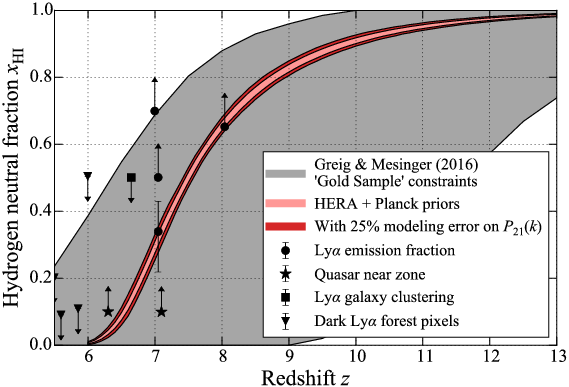
\includegraphics[width=1.\textwidth]{Koopmans_Bernardi/hera_ion_hist}
\end{center}
\caption{95\% confidence region on the Hydrogen neutral fraction $X_{\rm HI}$ (grey, from \cite{greig17}). The inclusion of HERA measurements leads to a dramatic improvement in the constraints (red and pink areas, \cite{liu16b}). Constraints from other reionization probes are shown as well (see \cite{deboer17} for a detailed description).}
\label{fig:fig_hera_ion_hist}
\end{figure}

Given the high redundant configuration, imaging tomography will remain challenging for HERA and likely the goal of a future generation experiment. As foreground modeling and characterization will also be limited because of redundancy and the coarse angular resolution, a significant effort was dedicated to keep the instrumental response from corrupting the intrinsically smooth foreground spectra and to accurately model it (\cite{neben16}, \cite{ewallwice16}, \cite{thyagarajan16}, \cite{patra18}). An alternative approach to redundant calibration is to apply foreground avoidance using closure phase quantities from antenna triads (\cite{thyagarajan18}): closure phase are insensitive to errors in direction independent interferometric calibration and, therefore, directly bypass the requirement of an accurate spectral calibration (see Chapter~\ref{chapter:bernardi} in this book for an overview of calibration of 21~cm observations). A preliminary analysis of HERA closure phases seem to confirm these premises (\cite{carilli18}).

HERA is currently under construction, with more than 200 dishes deployed, and 21~cm observations are currently being analyzed. New feeds that extend the sensitivity to the 50-250~MHz range are currently deployed for testing in order to enable observations in the $12 < z < 35$ range (the Cosmic Dawn) and probe the nature of the first luminous sources and their impact on the thermal history of the intergalacic medium.



\subsection{The Large aperture Experiment to detect the Dark Ages}
\label{section:leda_pspec}
\begin{figure}[]
\begin{center}
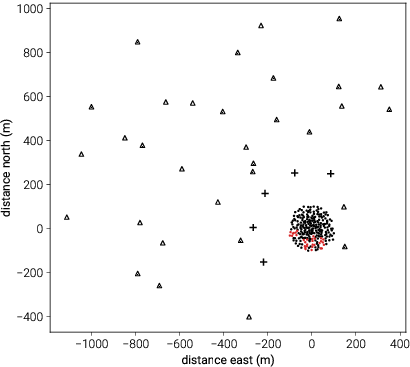
\includegraphics[width=1.\textwidth]{Koopmans_Bernardi/lwa_layout}
\end{center}
\caption{LEDA antenna layout: the dense core is surrounded by 32 dipoles in order to provide an exceptionally good instantaneous $uv$ coverage (from \cite{eastwood18}).}
\label{fig:fig_leda}
\end{figure}
The Large aperture Experiment to detect the Dark Ages (LEDA, \cite{bernardi15}, \cite{kocz15}) is located at the Owens Valley Radio Observatory, California. It operates in the 30-88~MHz frequency range, corresponding to $15 < z < 46$, seeking to detect the 21~cm signal from the Cosmic Dawn.   
The array layout consists of 251 dipoles pseudo randomly deployed within a 200~m diameter core, 23 dipoles are added out to a maximum 1.5~km baseline (see Figure~\ref{fig:fig_leda}). Five additional outrigger dipoles are custom-equipped to measure the global 21~cm signal via individual custom-built dipoles (see Section~\ref{leda_global}).

The very dense core provides exceptional brightness sensitivity and a point spread function with very low sidelobes. The outrigger dipoles improve the angular resolution that helps to identify calibration sources and lower the confusion level. As the dipoles are individually correlated, visibilities have contributions from all-sky emission, particularly from Galactic diffuse emission - given the number of short baselines - and with significant ionospheric-induced refraction and scintillation. Despite these challenges, \cite{eastwood18} generated the first high quality all-sky foreground maps. 

The LEDA approach to measure the 21~cm signal can be versatile, allowing to image and subtract foregrounds (\cite{eastwood18}) but also to avoid them (similar to \cite{beardsley16}). \cite{eastwood19} analyzed 20~hours of LEDA data calibrated using a compact source sky model and filtering foregrounds by using their statistical properties in way similar to \cite{dillon14} and \cite{trott16}. They reported an initial $10^8$~mK$^2$ upper limit on the 21~cm power spectrum at $z = 18.4$. Several hundreds of hours of observations have been collected now and will be the focus of future analysis towards the detection of the power spectrum from the Cosmic Dawn and an independent confirmation of the reported detection by \cite{bowman18}.



\subsection{The Low Frequency Array}
\label{section:lofar}



\subsection{The Murchison Widefield Array phase II}

Chapters~\ref{chapter:bernardi} and 8 have already described the relevant aspects of the MWA phase II upgrade. Here we emphasize the improved sensitivity to the 21~cm power spectrum due to the addition of the two redundant hexagon near to the core. Figure~\ref{fig:fig_mwa_phaseII_pspec} shows a sensitivity improvement of a factor of four with respect to the phase I and $\sim 10\sigma$ detection of the fiducial 21~cm power spectrum at $k \sim 0.1$~Mpc$^{-1}$. {\bf (GB: Leon, are you ok with this summary?)}
\begin{figure}[]
\begin{center}
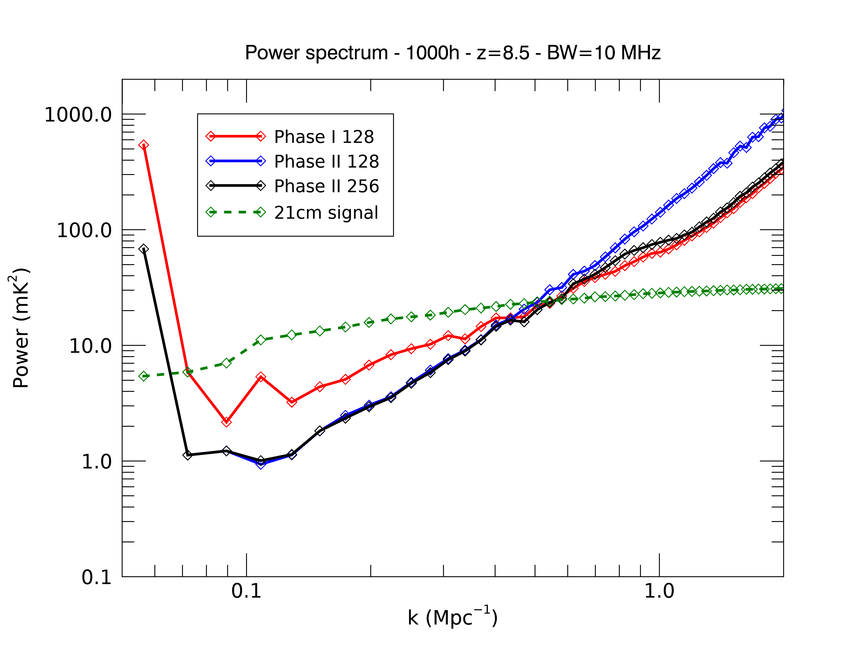
\includegraphics[width=1.\textwidth]{Koopmans_Bernardi/mwa_phaseII_pspec}
\end{center}
\caption{Fiducial 21~cm power spectrum model at $z = 8.5$ with associated noise levels from Phase I and Phase II arrays with a 1000~hour observation. ``Phase II 256" shows the result from a future MWA upgrade where all 256 tiles are correlated simultaneously (from \cite{wayth18}).}
\label{fig:fig_mwa_phaseII_pspec}
\end{figure}




\section{Forthcoming Global Signal Experiments}

In this Section we review the status of the ongoing global signal experiments (see Chapter~7 for a more detailed discussion about global signal observations).

\subsection{The Experiment to Detect the Global EoR Signature}
%\begin{figure}[]
%\begin{center}
%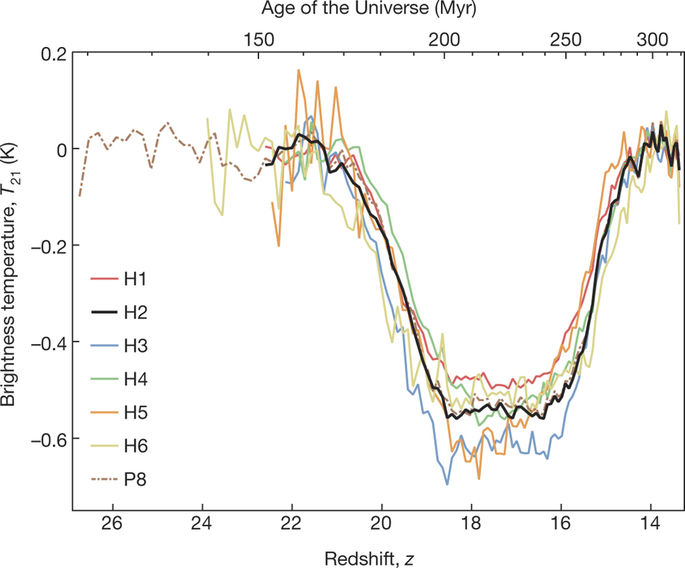
\includegraphics[width=1.\textwidth]{Koopmans_Bernardi/edges_trough}
%\end{center}
%\caption{EDGES}
%\label{fig:fig_edges}
%\end{figure}
The Experiment to Detect the Global EoR Signature (EDGES, \cite{bowman08} currently operates in two frequency bands: the $90-200$~MHz band (high band) in order to constrain the evolution of the neutral fraction throughout reionization, and the $50-100$~MHz band (low band), in order to measure the expected heating of the intergalactic medium from the primordial sources. 
The EDGES experiment has been pioneering techniques to accurately model all the various instrumental components in order to carefully control systematics effects. Observations in the high band have constrained the duration of reionization $\Delta z$ to be longer than $\Delta z >  1$ and started to constrain some properties of the first galaxies (\cite{monsalve17}, \cite{monsalve18}). In the low band, \cite{bowman18} reported the surprising detection of an absorption trough twice as deeper than the most extreme models, posing a serious challenge to its interpretation - assuming it is of cosmological issue. 

In the light of this anomalous signal, the EDGES team is deploying a new dipole antenna tuned in size to simultaneously observe the $60-160$~MHz range (i.e. $\sim 25\%$ smaller than the low band antenna) and confirm the results in the low band. A further upgrade of the EDGES experiment with a more portable antenna that includes the electronics is under consideration for deployment in a quiet radio frequency environment in Oregon, USA.



\subsection{The Large aperture Experiment to detect the Dark Ages: status and perspectives of global signal measurements}
\label{leda_global}
%\begin{figure}[]
%\begin{center}
%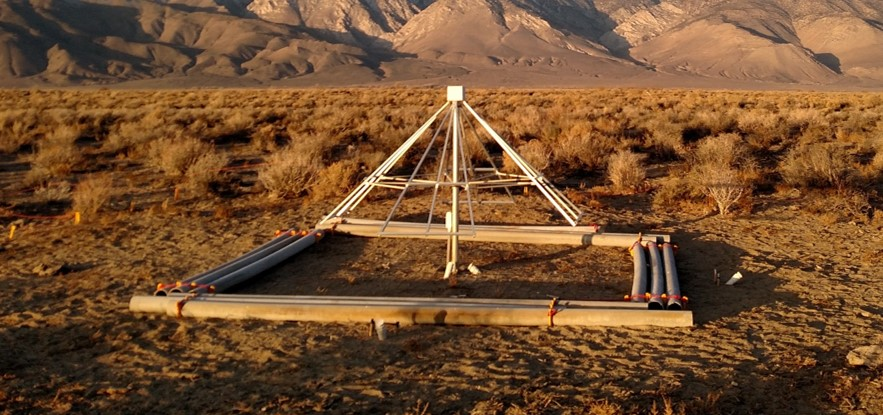
\includegraphics[width=1.\textwidth]{Koopmans_Bernardi/leda_dipole}
%\end{center}
%\caption{LEDA dipole}
%\label{fig:fig_leda_dipole}
%\end{figure}
As mentioned in Section~\ref{section:leda_pspec}, LEDA includes a few custom-equipped dipoles to measure the global signal (\cite{price18}, see also Chapter~7 in this book). Initial observations were used to validate the end-to-end acquisition system and data analysis, leading to a 890~mK upper limit on the global signal amplitude in the $13.2 < z < 27.4$ range at the 95\% confidence level (\cite{bernardi16}). A series of upgrades have been implemented since the early system: filters with a sharper roll-off were installed in order to improve RFI rejection and extend the observing band up to 87.5~MHz in order to validate the results by \cite{bowman18}; the stability of the noise diodes has been improved and a system to measure the ambient temperature at the antenna has been installed. The receiver seems to show the necessary stability to measure the global signal, however, other sources of systematics related to the antenna gain pattern remain lees well known and are the subject of ongoing modeling and investigation.

About 100~hours of observations were taken with the upgraded system and are currently being analyzed.

{\bf (GB: this section may be removed if already included in Chapter~7, I cannot see that chapter yet...)}


\section{Current and planned space based instruments}

\subsection{The Dark Ages Polarimetry Pathfinder}
The Dark Ages Polarimetry Pathfinder (DAPPER, \cite{burns19}) is a space satellite that is intended to observe the global signal from a $50 \times 125$~km lunar orbit, one of the quietest radio frequency environments, with an expected 26~month liftime. Its goal is to observe the global signal absorption trough that is expected at $35 < z < 80$, well before the formation of the first luminous sources (see Chapter~2 in this book). In this epoch, the global signal profile is purely determined by cosmology in the linear regime without being affected by complex astrophysical processes. DAPPER is expected to characterize the expected global signal, including any deviation that may be due by the additional cooling reported by \cite{bowman18}. Its strategy includes the use of a polarimeter to measure polarization induced by the anisotropic foregrounds and large antenna beam to aid in the separation of the foregrounds from the isotropic, unpolarized global signal (\cite{nhan17}) and a pattern recognition data analysis that is trained on realisti smulations of observed foregrounds, instrument systematics and the expected global signal (\cite{tauscher18}).

DAPPER is one of nine smal satellite missions selected by NASA to be further study for a possible launch in the next decade.

%We report on the results of a NASA-funded Astrophysics SmallSat concept study for a proposed lunar-orbiting experiment, the Dark Ages Polarimeter PathfindER (DAPPER), that is designed to observe the unexplored Dark Ages epoch of the early Universe. The Dark Ages, probed by the highly redshifted 21-cm neutral hydrogen global signal, is the ideal epoch for a new rigorous test of the standard LCDM cosmological model. DAPPER will search for divergences from the standard model that will indicate new physics such as heating or cooling produced by dark matter. A broad absorption trough in the redshifted 21-cm spectrum is expected during the Dark Ages, prior to the formation of the first stars and thus determined entirely by cosmological phenomena. DAPPER will observe this pristine epoch (17-38 MHz; z 83-36), and will measure the amplitude of the 21-cm spectrum to the level required to distinguish (at >5-\u03c3) the standard cosmological model from that of additional cooling derived from recent EDGES results. The main challenge of this measurement is the removal of bright foregrounds. DAPPER is designed to overcome this by utilizing two pioneering techniques: (1) a polarimeter to measure polarization induced by the anisotropic foregrounds and large antenna beam to aid in the separation of the foregrounds from the isotropic, unpolarized global signal, and (2) a pattern recognition analysis pipeline based on well-characterized training sets of foregrounds from sky observations, instrument systematics from simulations and laboratory measurements, and signals from theoretical predictions. End-to-end simulations of the DAPPER instrument including thermal noise, systematics from the spectrometer/polarimeter and the beam-averaged foreground, along with 21-cm models which include added cooling meet our sensitivity requirements to separate the standard cosmological models from ones that point toward new physics. DAPPER's science instrument consists of dual orthogonal dipole antennas and a tone-injection receiver based on high TRL components from the Parker Solar Probe/FIELDS, CURIE, and WIND/WAVES. DAPPER will be deployed into a frozen 50x125 km lunar orbit to provide 4615 hours of radio-quiet integration over a 26 month lifetime. 
%
%NASA recently picked the Dark Ages Polarimetry Pathfinder (DAPPER) as one of nine small satellite missions that it will study for a potential launch next decade. 

%\section{A Section}
%
%Lorem ipsum dolor sit amet, consectetur adipiscing elit. Duis eu egestas erat. Maecenas tincidunt lacinia tincidunt. Mauris id lectus nec neque feugiat condimentum vitae at diam. In vel orci nunc, non commodo mauris. Vivamus ipsum enim, vulputate quis pharetra non, molestie quis felis. Vivamus porttitor placerat turpis at accumsan. Nunc tortor velit, faucibus a rhoncus nec, blandit non elit. Nam consectetur lectus eu nisi blandit dapibus rhoncus dui tempus. Mauris fermentum dolor vel ipsum vulputate sit amet ultricies tortor lacinia. Donec ut nibh erat. Morbi nec mi ante. Integer nec vestibulum diam. Donec tincidunt pellentesque quam, ut interdum mauris venenatis condimentum. Nam condimentum, augue in aliquet gravida, neque dui elementum eros, id semper eros purus sed felis. Curabitur in justo sit amet sapien ultrices hendrerit at quis nibh. Quisque iaculis pulvinar tincidunt. 
%\begin{eqnarray}
%C(12) &= &\left[\overrightarrow{\pi}\cdot\overrightarrow{\phi}(x+r)\right] \nonumber \\ 
%&\approx& 1-\mathrm{const}\frac{r^2}{L^2}\int_r^L\frac{x\rmd x}{x^2} + \cdots \nonumber  \\
%&\approx& 1-\mathrm{const}\frac{r^2}{L^2}\ln\frac{x\rmd x}{x^2} + \cdots .\label{brokenlongeqn}
%\end{eqnarray}
%
%Aenean tellus risus, porta sit amet porta vitae, tincidunt ut felis. Class aptent taciti sociosqu ad litora torquent per conubia nostra, per inceptos himenaeos. Vestibulum ante ipsum primis in faucibus orci luctus et ultrices posuere cubilia Curae; Phasellus pulvinar placerat velit auctor egestas. Vivamus euismod fringilla tincidunt. Sed ut magna felis, id sollicitudin nunc. Quisque a dui eu erat consectetur egestas a quis justo. Aenean euismod congue diam, vel posuere urna fermentum sit amet. Lorem ipsum dolor sit amet, consectetur adipiscing elit. Mauris faucibus lacus eget est mollis auctor. Donec at nibh ligula, et posuere massa. Phasellus quis leo diam \cite{diamantaras1996pcn}.
%Donec aliquam blandit risus, eu venenatis ante euismod eu. Curabitur cursus justo id arcu condimentum feugiat. Integer sapien urna, vulputate et adipiscing nec, convallis et justo. Suspendisse in ipsum at felis ornare interdum \cite{tulone2006pts},
%
%\begin{figure}[]
%\begin{center}
%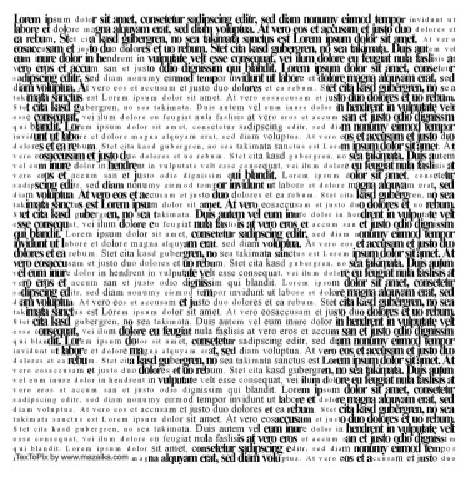
\includegraphics[width=0.5\textwidth]{Koopmans_Bernardi/01x01-eps-converted-to}
%\end{center}
%\caption{This is figure 1 in chapter 1.}
%\end{figure}
%
%\paragraph{Cras adipiscing} sagittis nunc vel luctus. Suspendisse volutpat augue quis erat semper consequat dignissim tellus euismod. Morbi hendrerit, tellus id aliquam iaculis, nibh leo tincidunt eros, vitae varius ligula felis in mi.
%
%\begin{table}
%\caption{Greek Letters.}
%\begin{center}
%\begin{tabular}{llllllll}
%\hline
%$\alpha $  & $ \beta $  & $ \gamma $  & $ \delta $  & $ \epsilon $  & $ \varepsilon $  & $ \zeta $  & $ \eta $ \\
% $ \theta $  &  $ \vartheta $  &  $ \gamma $  &  $ \kappa $  &  $ \lambda $  &  $ \mu $  &  $ \nu $  &  $ \xi $ \\
% $ o $  &  $ \pi $  &  $ \varpi $  &  $ \rho $  &  $ \varrho $  &  $ \sigma $  &  $ \varsigma $  &  $$ \\
% $ \tau $  &  $ \upsilon $  &  $ \phi$ &  $ \varphi $  &  $ \chi $  &  $ \psi $  &  $ \omega$  &  $ $ \\
% &  &  &  &  &  &  & \\
%$ \Gamma $  & $ \Delta $  & $ \Theta $  &  $ \Lambda $  &  $ \Xi $  &  $ \Pi $  &  $ \Sigma $  & $ \Upsilon $ \\
% $ \Phi$ &  $ \Psi $  &  $ \Omega $  &  &  &  &  &\\
%\hline
%\end{tabular}
%\end{center}\end{table}
%
%\begin{figure}[]
%\begin{center}
%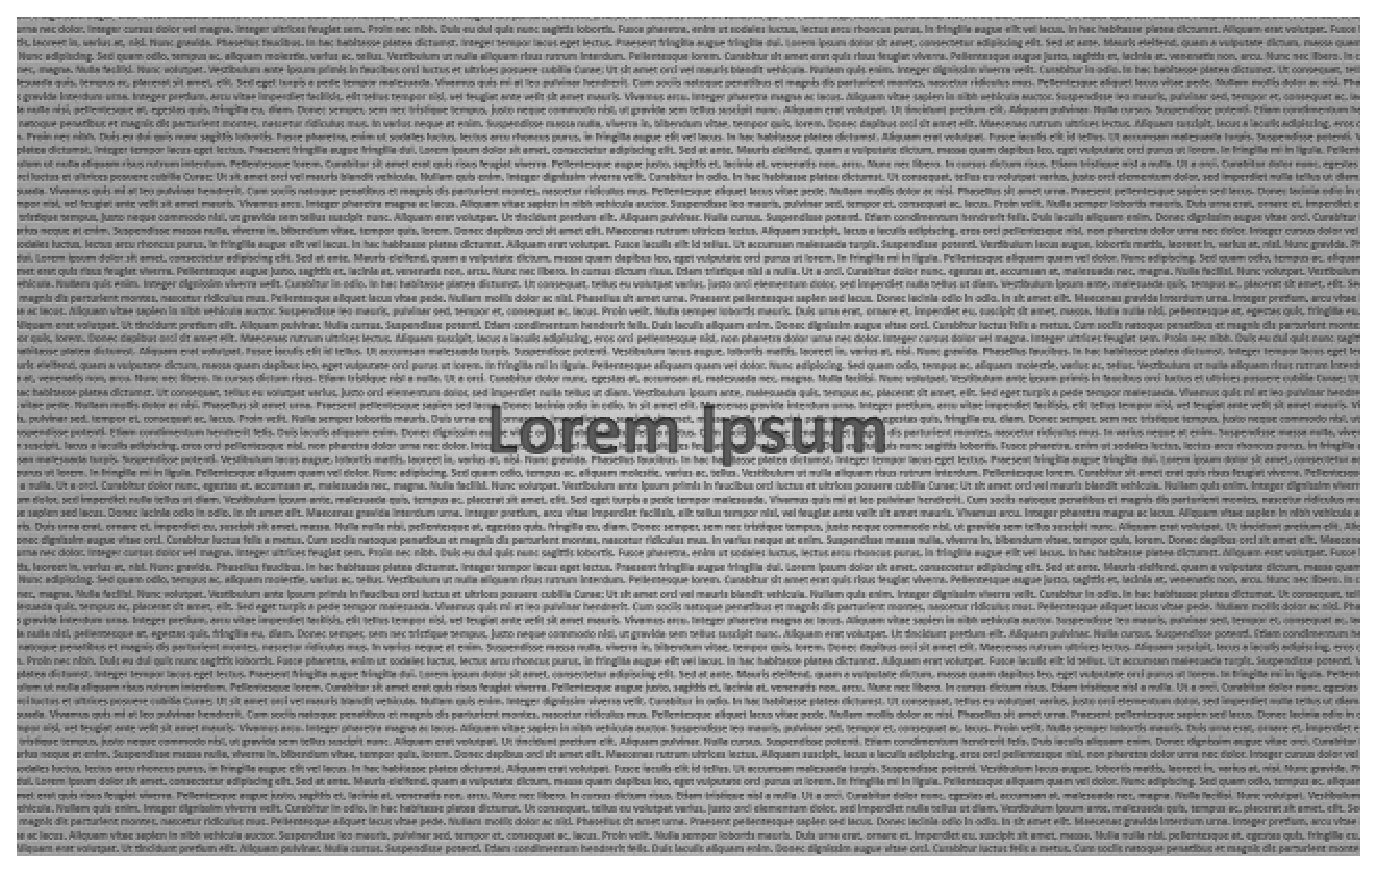
\includegraphics[width=0.6\textwidth]{Koopmans_Bernardi/01x02}
%\end{center}
%\caption{This is figure 2 in chapter 1.}
%\end{figure}


\bibliographystyle{plain}
\bibliography{Koopmans_Bernardi/References}


